\section{Transformation to Dual}
\label{sect:transformation-to-dual}

In the third phase, we take the filtered graph embedding and turn it into a valid map.

Formally speaking, the map we want to create is an area-proportional contact representation of the filtered graph embedding: The regions on the map correspond to the vertices of the filtered graph embedding and the clusters in the primal graph. Neighboring regions represent edges of the filtered graph embedding and the similarity of two clusters in the primal graph.

In this thesis we restrict ourselves to simple, polygonal contact representations, \ie{} contact representations in which the regions are polygons that don't intersect themselves. These contact representations can themselves be viewed as topological embeddings of a graph: A graph whose vertices are the endpoints of the polygonal areas and whose edges are the edges of the polygonal areas. We shall refer to this graph embedding as the \emph{boundary graph embedding}. The faces of this graph correspond to vertices in the filtered graph embedding and therefore inherit their weights.

The \emph{dual} of a plane graph $G$ is a pseudograph $G^*$ that has a vertex for each face in $G$, including the outer face, and edges connecting the vertices corresponding to the incident faces of each edge in the primal graph $G$. Forming the dual of a plane graph essentially turns vertices into faces and vice versa and \quoted{flips} the edges of the primal graph. When forming the dual of the dual of a plane graph, we get back the primal graph, \ie{} $(G^*)^* = G$.
%$G^*$ is a pseudograph because it can have loops and parallel edges.
%The dual $G^*$ of a plane graph $G$ is itself plane and an embedding can trivially be derived from an embedding of the primal graph $G$.

The \emph{weak dual} $G^-$ of a plane graph is its dual without the vertex corresponding to the primal outer face \cite{fleischner1974}. We define the \emph{augmented dual} $G^+$ of a plane graph $G$ as the pseudograph obtained by first adding a new vertex in the outer face of $G$ and connecting it to all vertices on the outer face and then forming the dual. By definition, the weak dual of the augmented dual of a plane graph is the primal graph again, \ie{} $(G^+)^- = G$ \cite{fleischner1974}.
\todo{Is there a known name for the inverse of \quoted{weak dual}? I couldn't find anything.}

Using the terminology from above, the filtered graph embedding is the weak dual of the boundary graph embedding with its degree-2-vertices smoothed out. In this phase of the pipeline, we aim to go in the opposite direction though: we are given a filtered graph embedding and want to create a corresponding boundary graph embedding with straight-line edges. We start by forming its augmented dual, as illustrated in the following figure:

\begin{figure}[H]
	\centering
	\subfigure[]{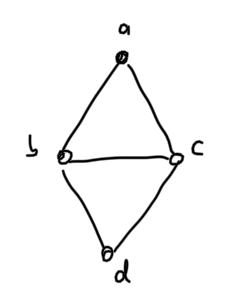
\includegraphics[height=40mm]{Resources/Transformation-1.png}}
	\subfigure[]{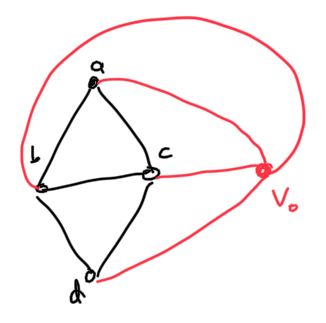
\includegraphics[height=40mm]{Resources/Transformation-2.png}}
	\subfigure[]{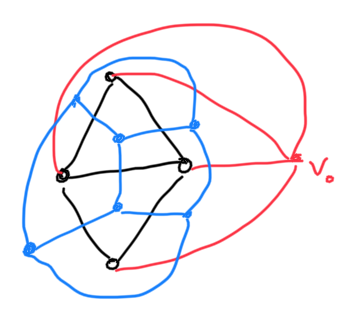
\includegraphics[height=40mm]{Resources/Transformation-3.png}}
	\subfigure[]{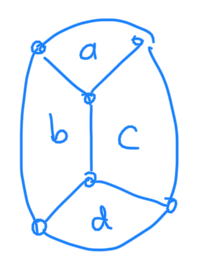
\includegraphics[height=40mm]{Resources/Transformation-5.png}}
	\caption{Step-by-step representation of the transformation from filtered graph embedding (a) to boundary graph embedding (d). We add the helper vertex in red (b) and form the dual in blue (c).}
	\label{fig:transformation}
\end{figure}

Since the boundary graph is supposed to have straight-line edges, we may need to tweak the embedding to straighten out the edges. The boundary graph is simple by definition, \ie{} it has no loops or parallel edges. Thus according to Fáry's theorem \cite{fary1948straight}, there exists a combinatorially isomorphic, straight-line re-embedding of the graph.

Thomassen proved that there exist straight-line drawings of all plane cubic graphs with arbitrary prescribed face areas \cite{thomassen1992plane}. Adding a new vertex in the outer face of an internally triangulated graph and connecting it to all vertices on the outer face creates a fully triangulated graph, and its dual is a cubic (3-regular) graph. Therefore \cite{thomassen1992plane} applies to our boundary graph, meaning that even without any subdivisions there exists an embedding that realizes the face weights, \ie{} a map with perfect statistical accuracy.
% We only need Kleist when lifting restrictions and our graph isn't necessarily cubic.

Such embeddings are non-trivial to find though and may create undesired regions for other quality metrics that we want to optimize for. Concrete implementations of this phase are in no way required to use triangles for all map regions and are free to subdivide edges at will. In fact, we provide a very simple implementation that subdivides all dual edges once and leaves us with enough degrees of freedom to optimize for other quality metrics in \cref{chap:implementation}.

\begin{figure}[H]
	\centering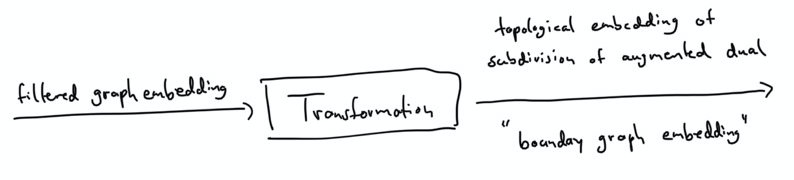
\includegraphics[width=0.9\textwidth]{Resources/Pipeline-Transformation.png}
	\caption{Input and output of the transformation phase.}
	\label{fig:pipeline-transformation}
\end{figure}
